
%% bare_jrnl_compsoc.tex
%% V1.4b
%% 2015/08/26
%% by Michael Shell
%% See:
%% http://www.michaelshell.org/
%% for current contact information.
%%
%% This is a skeleton file demonstrating the use of IEEEtran.cls
%% (requires IEEEtran.cls version 1.8b or later) with an IEEE
%% Computer Society journal paper.
%%
%% Support sites:
%% http://www.michaelshell.org/tex/ieeetran/
%% http://www.ctan.org/pkg/ieeetran
%% and
%% http://www.ieee.org/

%%*************************************************************************
%% Legal Notice:
%% This code is offered as-is without any warranty either expressed or
%% implied; without even the implied warranty of MERCHANTABILITY or
%% FITNESS FOR A PARTICULAR PURPOSE! 
%% User assumes all risk.
%% In no event shall the IEEE or any contributor to this code be liable for
%% any damages or losses, including, but not limited to, incidental,
%% consequential, or any other damages, resulting from the use or misuse
%% of any information contained here.
%%
%% All comments are the opinions of their respective authors and are not
%% necessarily endorsed by the IEEE.
%%
%% This work is distributed under the LaTeX Project Public License (LPPL)
%% ( http://www.latex-project.org/ ) version 1.3, and may be freely used,
%% distributed and modified. A copy of the LPPL, version 1.3, is included
%% in the base LaTeX documentation of all distributions of LaTeX released
%% 2003/12/01 or later.
%% Retain all contribution notices and credits.
%% ** Modified files should be clearly indicated as such, including  **
%% ** renaming them and changing author support contact information. **
%%*************************************************************************


% *** Authors should verify (and, if needed, correct) their LaTeX system  ***
% *** with the testflow diagnostic prior to trusting their LaTeX platform ***
% *** with production work. The IEEE's font choices and paper sizes can   ***
% *** trigger bugs that do not appear when using other class files.       ***                          ***
% The testflow support page is at:
% http://www.michaelshell.org/tex/testflow/


\documentclass[10pt,journal,compsoc]{IEEEtran}
%
% If IEEEtran.cls has not been installed into the LaTeX system files,
% manually specify the path to it like:
% \documentclass[10pt,journal,compsoc]{../sty/IEEEtran}





% Some very useful LaTeX packages include:
% (uncomment the ones you want to load)


% *** MISC UTILITY PACKAGES ***
%
%\usepackage{ifpdf}
% Heiko Oberdiek's ifpdf.sty is very useful if you need conditional
% compilation based on whether the output is pdf or dvi.
% usage:
% \ifpdf
%   % pdf code
% \else
%   % dvi code
% \fi
% The latest version of ifpdf.sty can be obtained from:
% http://www.ctan.org/pkg/ifpdf
% Also, note that IEEEtran.cls V1.7 and later provides a builtin
% \ifCLASSINFOpdf conditional that works the same way.
% When switching from latex to pdflatex and vice-versa, the compiler may
% have to be run twice to clear warning/error messages.






% *** CITATION PACKAGES ***
%
\ifCLASSOPTIONcompsoc
  % IEEE Computer Society needs nocompress option
  % requires cite.sty v4.0 or later (November 2003)
  \usepackage[nocompress]{cite}
\else
  % normal IEEE
  \usepackage{cite}
\fi
% cite.sty was written by Donald Arseneau
% V1.6 and later of IEEEtran pre-defines the format of the cite.sty package
% \cite{} output to follow that of the IEEE. Loading the cite package will
% result in citation numbers being automatically sorted and properly
% "compressed/ranged". e.g., [1], [9], [2], [7], [5], [6] without using
% cite.sty will become [1], [2], [5]--[7], [9] using cite.sty. cite.sty's
% \cite will automatically add leading space, if needed. Use cite.sty's
% noadjust option (cite.sty V3.8 and later) if you want to turn this off
% such as if a citation ever needs to be enclosed in parenthesis.
% cite.sty is already installed on most LaTeX systems. Be sure and use
% version 5.0 (2009-03-20) and later if using hyperref.sty.
% The latest version can be obtained at:
% http://www.ctan.org/pkg/cite
% The documentation is contained in the cite.sty file itself.
%
% Note that some packages require special options to format as the Computer
% Society requires. In particular, Computer Society  papers do not use
% compressed citation ranges as is done in typical IEEE papers
% (e.g., [1]-[4]). Instead, they list every citation separately in order
% (e.g., [1], [2], [3], [4]). To get the latter we need to load the cite
% package with the nocompress option which is supported by cite.sty v4.0
% and later. Note also the use of a CLASSOPTION conditional provided by
% IEEEtran.cls V1.7 and later.





% *** GRAPHICS RELATED PACKAGES ***
%
\ifCLASSINFOpdf
  \usepackage[pdftex]{graphicx}
  % declare the path(s) where your graphic files are
  % \graphicspath{{../pdf/}{../jpeg/}}
   \graphicspath{{figures/}}
  % and their extensions so you won't have to specify these with
  % every instance of \includegraphics
  % \DeclareGraphicsExtensions{.pdf,.jpeg,.png}
\else
  % or other class option (dvipsone, dvipdf, if not using dvips). graphicx
  % will default to the driver specified in the system graphics.cfg if no
  % driver is specified.
  % \usepackage[dvips]{graphicx}
  % declare the path(s) where your graphic files are
  % \graphicspath{{../eps/}}
  % and their extensions so you won't have to specify these with
  % every instance of \includegraphics
  % \DeclareGraphicsExtensions{.eps}
\fi
% graphicx was written by David Carlisle and Sebastian Rahtz. It is
% required if you want graphics, photos, etc. graphicx.sty is already
% installed on most LaTeX systems. The latest version and documentation
% can be obtained at: 
% http://www.ctan.org/pkg/graphicx
% Another good source of documentation is "Using Imported Graphics in
% LaTeX2e" by Keith Reckdahl which can be found at:
% http://www.ctan.org/pkg/epslatex
%
% latex, and pdflatex in dvi mode, support graphics in encapsulated
% postscript (.eps) format. pdflatex in pdf mode supports graphics
% in .pdf, .jpeg, .png and .mps (metapost) formats. Users should ensure
% that all non-photo figures use a vector format (.eps, .pdf, .mps) and
% not a bitmapped formats (.jpeg, .png). The IEEE frowns on bitmapped formats
% which can result in "jaggedy"/blurry rendering of lines and letters as
% well as large increases in file sizes.
%
% You can find documentation about the pdfTeX application at:
% http://www.tug.org/applications/pdftex






% *** MATH PACKAGES ***
%
%\usepackage{amsmath}
% A popular package from the American Mathematical Society that provides
% many useful and powerful commands for dealing with mathematics.
%
% Note that the amsmath package sets \interdisplaylinepenalty to 10000
% thus preventing page breaks from occurring within multiline equations. Use:
%\interdisplaylinepenalty=2500
% after loading amsmath to restore such page breaks as IEEEtran.cls normally
% does. amsmath.sty is already installed on most LaTeX systems. The latest
% version and documentation can be obtained at:
% http://www.ctan.org/pkg/amsmath





% *** SPECIALIZED LIST PACKAGES ***
%
%\usepackage{algorithmic}
% algorithmic.sty was written by Peter Williams and Rogerio Brito.
% This package provides an algorithmic environment fo describing algorithms.
% You can use the algorithmic environment in-text or within a figure
% environment to provide for a floating algorithm. Do NOT use the algorithm
% floating environment provided by algorithm.sty (by the same authors) or
% algorithm2e.sty (by Christophe Fiorio) as the IEEE does not use dedicated
% algorithm float types and packages that provide these will not provide
% correct IEEE style captions. The latest version and documentation of
% algorithmic.sty can be obtained at:
% http://www.ctan.org/pkg/algorithms
% Also of interest may be the (relatively newer and more customizable)
% algorithmicx.sty package by Szasz Janos:
% http://www.ctan.org/pkg/algorithmicx




% *** ALIGNMENT PACKAGES ***
%
%\usepackage{array}
% Frank Mittelbach's and David Carlisle's array.sty patches and improves
% the standard LaTeX2e array and tabular environments to provide better
% appearance and additional user controls. As the default LaTeX2e table
% generation code is lacking to the point of almost being broken with
% respect to the quality of the end results, all users are strongly
% advised to use an enhanced (at the very least that provided by array.sty)
% set of table tools. array.sty is already installed on most systems. The
% latest version and documentation can be obtained at:
% http://www.ctan.org/pkg/array


% IEEEtran contains the IEEEeqnarray family of commands that can be used to
% generate multiline equations as well as matrices, tables, etc., of high
% quality.




% *** SUBFIGURE PACKAGES ***
%\ifCLASSOPTIONcompsoc
%  \usepackage[caption=false,font=footnotesize,labelfont=sf,textfont=sf]{subfig}
%\else
%  \usepackage[caption=false,font=footnotesize]{subfig}
%\fi
% subfig.sty, written by Steven Douglas Cochran, is the modern replacement
% for subfigure.sty, the latter of which is no longer maintained and is
% incompatible with some LaTeX packages including fixltx2e. However,
% subfig.sty requires and automatically loads Axel Sommerfeldt's caption.sty
% which will override IEEEtran.cls' handling of captions and this will result
% in non-IEEE style figure/table captions. To prevent this problem, be sure
% and invoke subfig.sty's "caption=false" package option (available since
% subfig.sty version 1.3, 2005/06/28) as this is will preserve IEEEtran.cls
% handling of captions.
% Note that the Computer Society format requires a sans serif font rather
% than the serif font used in traditional IEEE formatting and thus the need
% to invoke different subfig.sty package options depending on whether
% compsoc mode has been enabled.
%
% The latest version and documentation of subfig.sty can be obtained at:
% http://www.ctan.org/pkg/subfig




% *** FLOAT PACKAGES ***
%
%\usepackage{fixltx2e}
% fixltx2e, the successor to the earlier fix2col.sty, was written by
% Frank Mittelbach and David Carlisle. This package corrects a few problems
% in the LaTeX2e kernel, the most notable of which is that in current
% LaTeX2e releases, the ordering of single and double column floats is not
% guaranteed to be preserved. Thus, an unpatched LaTeX2e can allow a
% single column figure to be placed prior to an earlier double column
% figure.
% Be aware that LaTeX2e kernels dated 2015 and later have fixltx2e.sty's
% corrections already built into the system in which case a warning will
% be issued if an attempt is made to load fixltx2e.sty as it is no longer
% needed.
% The latest version and documentation can be found at:
% http://www.ctan.org/pkg/fixltx2e


%\usepackage{stfloats}
% stfloats.sty was written by Sigitas Tolusis. This package gives LaTeX2e
% the ability to do double column floats at the bottom of the page as well
% as the top. (e.g., "\begin{figure*}[!b]" is not normally possible in
% LaTeX2e). It also provides a command:
%\fnbelowfloat
% to enable the placement of footnotes below bottom floats (the standard
% LaTeX2e kernel puts them above bottom floats). This is an invasive package
% which rewrites many portions of the LaTeX2e float routines. It may not work
% with other packages that modify the LaTeX2e float routines. The latest
% version and documentation can be obtained at:
% http://www.ctan.org/pkg/stfloats
% Do not use the stfloats baselinefloat ability as the IEEE does not allow
% \baselineskip to stretch. Authors submitting work to the IEEE should note
% that the IEEE rarely uses double column equations and that authors should try
% to avoid such use. Do not be tempted to use the cuted.sty or midfloat.sty
% packages (also by Sigitas Tolusis) as the IEEE does not format its papers in
% such ways.
% Do not attempt to use stfloats with fixltx2e as they are incompatible.
% Instead, use Morten Hogholm'a dblfloatfix which combines the features
% of both fixltx2e and stfloats:
%
% \usepackage{dblfloatfix}
% The latest version can be found at:
% http://www.ctan.org/pkg/dblfloatfix




%\ifCLASSOPTIONcaptionsoff
%  \usepackage[nomarkers]{endfloat}
% \let\MYoriglatexcaption\caption
% \renewcommand{\caption}[2][\relax]{\MYoriglatexcaption[#2]{#2}}
%\fi
% endfloat.sty was written by James Darrell McCauley, Jeff Goldberg and 
% Axel Sommerfeldt. This package may be useful when used in conjunction with 
% IEEEtran.cls'  captionsoff option. Some IEEE journals/societies require that
% submissions have lists of figures/tables at the end of the paper and that
% figures/tables without any captions are placed on a page by themselves at
% the end of the document. If needed, the draftcls IEEEtran class option or
% \CLASSINPUTbaselinestretch interface can be used to increase the line
% spacing as well. Be sure and use the nomarkers option of endfloat to
% prevent endfloat from "marking" where the figures would have been placed
% in the text. The two hack lines of code above are a slight modification of
% that suggested by in the endfloat docs (section 8.4.1) to ensure that
% the full captions always appear in the list of figures/tables - even if
% the user used the short optional argument of \caption[]{}.
% IEEE papers do not typically make use of \caption[]'s optional argument,
% so this should not be an issue. A similar trick can be used to disable
% captions of packages such as subfig.sty that lack options to turn off
% the subcaptions:
% For subfig.sty:
% \let\MYorigsubfloat\subfloat
% \renewcommand{\subfloat}[2][\relax]{\MYorigsubfloat[]{#2}}
% However, the above trick will not work if both optional arguments of
% the \subfloat command are used. Furthermore, there needs to be a
% description of each subfigure *somewhere* and endfloat does not add
% subfigure captions to its list of figures. Thus, the best approach is to
% avoid the use of subfigure captions (many IEEE journals avoid them anyway)
% and instead reference/explain all the subfigures within the main caption.
% The latest version of endfloat.sty and its documentation can obtained at:
% http://www.ctan.org/pkg/endfloat
%
% The IEEEtran \ifCLASSOPTIONcaptionsoff conditional can also be used
% later in the document, say, to conditionally put the References on a 
% page by themselves.




% *** PDF, URL AND HYPERLINK PACKAGES ***
%
%\usepackage{url}
% url.sty was written by Donald Arseneau. It provides better support for
% handling and breaking URLs. url.sty is already installed on most LaTeX
% systems. The latest version and documentation can be obtained at:
% http://www.ctan.org/pkg/url
% Basically, \url{my_url_here}.





% *** Do not adjust lengths that control margins, column widths, etc. ***
% *** Do not use packages that alter fonts (such as pslatex).         ***
% There should be no need to do such things with IEEEtran.cls V1.6 and later.
% (Unless specifically asked to do so by the journal or conference you plan
% to submit to, of course. )


% correct bad hyphenation here
\hyphenation{op-tical net-works semi-conduc-tor}


\begin{document}
%
% paper title
% Titles are generally capitalized except for words such as a, an, and, as,
% at, but, by, for, in, nor, of, on, or, the, to and up, which are usually
% not capitalized unless they are the first or last word of the title.
% Linebreaks \\ can be used within to get better formatting as desired.
% Do not put math or special symbols in the title.
\title{Test}
%
%
% author names and IEEE memberships
% note positions of commas and nonbreaking spaces ( ~ ) LaTeX will not break
% a structure at a ~ so this keeps an author's name from being broken across
% two lines.
% use \thanks{} to gain access to the first footnote area
% a separate \thanks must be used for each paragraph as LaTeX2e's \thanks
% was not built to handle multiple paragraphs
%
%
%\IEEEcompsocitemizethanks is a special \thanks that produces the bulleted
% lists the Computer Society journals use for "first footnote" author
% affiliations. Use \IEEEcompsocthanksitem which works much like \item
% for each affiliation group. When not in compsoc mode,
% \IEEEcompsocitemizethanks becomes like \thanks and
% \IEEEcompsocthanksitem becomes a line break with idention. This
% facilitates dual compilation, although admittedly the differences in the
% desired content of \author between the different types of papers makes a
% one-size-fits-all approach a daunting prospect. For instance, compsoc 
% journal papers have the author affiliations above the "Manuscript
% received ..."  text while in non-compsoc journals this is reversed. Sigh.


\author{xxx% <-this % stops a space
        }
%\author{Michael~Shell,~\IEEEmembership{Member,~IEEE,}
%        John~Doe,~\IEEEmembership{Fellow,~OSA,}
%        and~Jane~Doe,~\IEEEmembership{Life~Fellow,~IEEE}% <-this % stops a space
%\IEEEcompsocitemizethanks{\IEEEcompsocthanksitem M. Shell was with the Department
%of Electrical and Computer Engineering, Georgia Institute of Technology, Atlanta,
%GA, 30332.\protect\\
%% note need leading \protect in front of \\ to get a newline within \thanks as
%% \\ is fragile and will error, could use \hfil\break instead.
%E-mail: see http://www.michaelshell.org/contact.html
%\IEEEcompsocthanksitem J. Doe and J. Doe are with Anonymous University.}% <-this % stops an unwanted space
%\thanks{Manuscript received April 19, 2005; revised August 26, 2015.}}

% note the % following the last \IEEEmembership and also \thanks - 
% these prevent an unwanted space from occurring between the last author name
% and the end of the author line. i.e., if you had this:
% 
% \author{....lastname \thanks{...} \thanks{...} }
%                     ^------------^------------^----Do not want these spaces!
%
% a space would be appended to the last name and could cause every name on that
% line to be shifted left slightly. This is one of those "LaTeX things". For
% instance, "\textbf{A} \textbf{B}" will typeset as "A B" not "AB". To get
% "AB" then you have to do: "\textbf{A}\textbf{B}"
% \thanks is no different in this regard, so shield the last } of each \thanks
% that ends a line with a % and do not let a space in before the next \thanks.
% Spaces after \IEEEmembership other than the last one are OK (and needed) as
% you are supposed to have spaces between the names. For what it is worth,
% this is a minor point as most people would not even notice if the said evil
% space somehow managed to creep in.



% The paper headers
\markboth{Journal of \LaTeX\ Class Files,~Vol.~14, No.~8, August~2015}%
{Shell \MakeLowercase{\textit{et al.}}: Bare Demo of IEEEtran.cls for Computer Society Journals}
% The only time the second header will appear is for the odd numbered pages
% after the title page when using the twoside option.
% 
% *** Note that you probably will NOT want to include the author's ***
% *** name in the headers of peer review papers.                   ***
% You can use \ifCLASSOPTIONpeerreview for conditional compilation here if
% you desire.



% The publisher's ID mark at the bottom of the page is less important with
% Computer Society journal papers as those publications place the marks
% outside of the main text columns and, therefore, unlike regular IEEE
% journals, the available text space is not reduced by their presence.
% If you want to put a publisher's ID mark on the page you can do it like
% this:
%\IEEEpubid{0000--0000/00\$00.00~\copyright~2015 IEEE}
% or like this to get the Computer Society new two part style.
%\IEEEpubid{\makebox[\columnwidth]{\hfill 0000--0000/00/\$00.00~\copyright~2015 IEEE}%
%\hspace{\columnsep}\makebox[\columnwidth]{Published by the IEEE Computer Society\hfill}}
% Remember, if you use this you must call \IEEEpubidadjcol in the second
% column for its text to clear the IEEEpubid mark (Computer Society jorunal
% papers don't need this extra clearance.)



% use for special paper notices
%\IEEEspecialpapernotice{(Invited Paper)}



% for Computer Society papers, we must declare the abstract and index terms
% PRIOR to the title within the \IEEEtitleabstractindextext IEEEtran
% command as these need to go into the title area created by \maketitle.
% As a general rule, do not put math, special symbols or citations
% in the abstract or keywords.
\IEEEtitleabstractindextext{%
\begin{abstract}

\cite{Zhang2018}
Accurate application classification is important and useful to improve network
performance. However, with the continuous expansion of network scale and the
rapid increase of network users, it is very difficult for the existing application
classification methods to accurately identify and classify network applications.
Currently, most classification methods are suitable for small-scale data sets
and cannot achieve high classification accuracy because of the shallow learn-
ing structure and the limited learning ability. The emergence of deep learning
technology and software-defined networking (SDN) enables the application
classification method to process large-scale data.  In this paper, by leveraging
the SDN architecture, we present a novel hybrid deep neural network–based
application classification method, which achieves high classification accuracy
without the manual feature selection and extraction. In the proposed applica-
tion classification framework, by taking the advantage of the logical centralized
control and powerful computing capability, the massive network traffic is eas-
ily collected and processed by the SDN controller. The processed data is used to
train the hybrid deep neural network, which is composed of the stacked autoen-
coder and softmax regression layer. The deep flow features can be obtained from
the stacked autoencoder automatically instead of the manual feature selection
and extraction. The softmax regression layer is used as the classifier to realize the
application classification. Finally, simulation results demonstrate that our pro-
posed classification method is effective and gets higher classification accuracy
than the support vector machine–based classification method

As well known, accurate network application classification is important and useful for many network activities such
as network management, quality-of-service (QoS) provisioning, network security, and intrusion detection.
1 Networkapplication classification classifies different network traffic and divides the traffic into different classes. To achieve accu- rate network applications, a large number of different application classification methods have been proposed in the past
few decades, mainly including port-based approach, payload-based approach, and machine learning–based approach.
2
In
current years, the most widely used technology for application classification is the machine learning–based approach, in
which backpropagation (BP) neural network, Bayesian network, support vector machine (SVM), and C4.5 decision tree
are usually applied to the classification.
3-11
Different from identifying port number in the port-based approach as well as inspecting payload content in the
payload-based approach, in machine learning–based classification methods, the flow features statistics, including the
size of packet, interpacket time, and flow duration time, are used to automatically identify and classify network applica-
tion by using machine learning. The shallow neural network is generally used to build the application classifier in lots of
machine learning–based classification methods. The shallow neural network has limited feature learning ability because
of few nonlinear feature extraction layers, and it is more suitable to deal with small-scale data problems. However, with
the constant enlargement of network scale and the coming of the big data era, network traffic explosively grows, and large
amounts of novel network applications have generated. It is very challenging for traditional shallow neural network–based
classification method to deal with massive network traffic because of the limited feature learning ability. In order to extract
deep feature and obtain high-level feature presentation from a large-scale data set, deep learning network is required.
Recently, deep learning has been proposed, and some deep neural network models, for example, stacked autoencoder,
convolutional neural network (CNN), and deep belief network (DBN), have been widely applied in many fields such as
classification, speech recognition, and natural language processing.
12
Deep learning is a novel machine learning algorithm
that is used to train deeper neural networks. By contrast, traditional learning algorithm, which is adopted to train shallow
neural networks, is not suitable for training deep neural networks because of the reason of easily getting stuck in local
optima and diffusion of gradient.
13
Compared with traditional shallow neural networks, deep neural networks contain
multiple hidden layers such that it has the stronger nonlinear feature extraction ability to achieve the higher level or more
complex feature presentation. Meanwhile, deep neural networks have the ability of yielding higher classification accuracy
than shallow neural networks. Hence, in this paper, we propose a novel classification method on the basis of the hybrid
deep learning network model.


 Network Traffic Classifier (NTC) is an important
part of current network monitoring systems, being its task to infer the network service that is currently used by a communication flow (e.g. HTTP, SIP…). The detection is based on a number of features associated with the communication flow, for example, source and destination ports and bytes transmitted per packet. NTC is important because much information about a current network flow can be learned and anticipated just by knowing its network service (required latency, traffic volume, possible duration…). This is of particular interest for the management and monitoring of Internet of Things (IoT) networks, where NTC will help to segregate traffic and behavior of heterogeneous devices and services. In this paper, we present a new technique for NTC based on a combination of deep learning models that can be used for IoT traffic. We show that a Recurrent Neural Network (RNN) combined with a Convolutional Neural Network (CNN) provides best detection results. The natural domain for a CNN, which is image processing, has been extended to NTC in an easy and natural way. We show that the proposed method provides better detection results than alternative algorithms without requiring any feature engineering, which is usual when applying other models. A complete study is presented on several architectures that integrate a CNN and an RNN, including the impact of the features chosen and the length of the network flows used for training.
\end{abstract}

% Note that keywords are not normally used for peerreview papers.
\begin{IEEEkeywords}
%% Computer Society, IEEE, IEEEtran, journal, \LaTeX, paper, template.
    Application classification, Encrypted traffic classification, LSTM, CNN
\end{IEEEkeywords}}


% make the title area
\maketitle


% To allow for easy dual compilation without having to reenter the
% abstract/keywords data, the \IEEEtitleabstractindextext text will
% not be used in maketitle, but will appear (i.e., to be "transported")
% here as \IEEEdisplaynontitleabstractindextext when the compsoc 
% or transmag modes are not selected <OR> if conference mode is selected 
% - because all conference papers position the abstract like regular
% papers do.
\IEEEdisplaynontitleabstractindextext
% \IEEEdisplaynontitleabstractindextext has no effect when using
% compsoc or transmag under a non-conference mode.



% For peer review papers, you can put extra information on the cover
% page as needed:
% \ifCLASSOPTIONpeerreview
% \begin{center} \bfseries EDICS Category: 3-BBND \end{center}
% \fi
%
% For peerreview papers, this IEEEtran command inserts a page break and
% creates the second title. It will be ignored for other modes.
\IEEEpeerreviewmaketitle



\IEEEraisesectionheading{\section{Introduction}\label{sec:introduction}}
%% Computer Society journal (but not conference!) papers do something unusual
%% with the very first section heading (almost always called "Introduction").
%% They place it ABOVE the main text! IEEEtran.cls does not automatically do
%% this for you, but you can achieve this effect with the provided
%% \IEEEraisesectionheading{} command. Note the need to keep any \label that
%% is to refer to the section immediately after \section in the above as
%% \IEEEraisesectionheading puts \section within a raised box.
%
%
%
%
%% The very first letter is a 2 line initial drop letter followed
%% by the rest of the first word in caps (small caps for compsoc).
%% 
%% form to use if the first word consists of a single letter:
%% \IEEEPARstart{A}{demo} file is ....
%% 
%% form to use if you need the single drop letter followed by
%% normal text (unknown if ever used by the IEEE):
%% \IEEEPARstart{A}{}demo file is ....
%% 
%% Some journals put the first two words in caps:
%% \IEEEPARstart{T}{his demo} file is ....
%% 
%% Here we have the typical use of a "T" for an initial drop letter
%% and "HIS" in caps to complete the first word.
%\IEEEPARstart{T}{his} demo file is intended to serve as a ``starter file''
%for IEEE Computer Society journal papers produced under \LaTeX\ using
%IEEEtran.cls version 1.8b and later.
%% You must have at least 2 lines in the paragraph with the drop letter
%% (should never be an issue)
%I wish you the best of success.



\cite{Shen2017}
With a profusion of network applications, traf-
fic classification plays a crucial role in network management and policy-based security control. The widely used encryption transmission protocols, such as the secure socket layer/transport layer security (SSL/TLS) protocols, lead to the failure of tradi- tional payload-based classification methods. Existing methods for encrypted traffic classification cannot achieve high discrimination accuracy for applications with similar fingerprints. Ins. In this paper, we propose an attribute-aware encrypted traffic classification method based on the second-order Markov Chains. We start by exploring approaches that can further improve the perfor- mance of existing methods in terms of discrimination accuracy, and make promising observations that the application attribute bigram, which consists of the certificate packet length and the first application data size in SSL/TLS sessions, contributes to application discrimination. To increase the diversity of applica- tion fingerprints, we develop a new method by incorporating the attribute bigrams into the second-order homogeneous Markov chains. Extensive evaluation results show that the proposed method can improve the classification accuracy by 29% on the average compared with the state-of-the-art Markov-based method

NETWORK traffic is composed of packets carrying data belonging to a variety of applications. Classification of
traffic helps network operators to identify specific applications and protocols that exist in a network, which can be useful for many different purposes [19], [32], [33], such as network planning, application prioritization for QoS guarantees, and
policy deployment for security control. For instance, a network operator might want to assign traffic from known popular applications with a higher priority for better user experience, and an enterprise network operator might block traffic from a given application by means of application-level firewalls. Traditional traffic classification techniques are often
designed based on the analysis of packet contents, such as the port-based methods and the payload-based methods. In recent years we have seen a dramatic growth in the usage of encryp- tion protocols, such as the SSL/TLS protocols [13], [16]. Since packet payloads are encrypted, these methods can no longer fulfil efficient recognition. Therefore, it is desirable to develop classification methods for encrypted traffic [12]. Korczynski and Duda proposed such a method by using the

  \cite{Lopez-Martin2017}
A Network Traffic Classifier (NTC) is an important
part of current network monitoring systems, being its task to infer the network service that is currently used by a communication flow (e.g. HTTP, SIP…). The detection is based on a number of features associated with the communication flow, for example, source and destination ports and bytes transmitted per packet. NTC is important because much information about a current network flow can be learned and anticipated just by knowing its network service (required latency, traffic volume, possible duration…). This is of particular interest for the management and monitoring of Internet of Things (IoT) networks, where NTC will help to segregate traffic and behavior of heterogeneous devices and services. In this paper, we present a new technique for NTC based on a combination of deep learning models that can be used for IoT traffic. We show that a Recurrent Neural Network (RNN) combined with a Convolutional Neural Network (CNN) provides best detection results. The natural domain for a CNN, which is image processing, has been extended to NTC in an easy and natural way. We show that the proposed method provides better detection results than alternative algorithms without requiring any feature engineering, which is usual when applying other models. A complete study is presented on several architectures that integrate a CNN and an RNN, including the impact of the features chosen and the length of the network flows used for training.

\cite{Taylor2018}
Much work has been done on analysing traffic from work-
stations and web browsers [4]. At first glance, fingerprinting smartphone apps may seem to be a simple translation of exist- ing work. While there are some similarities, there are nuances in the type of traffic sent by smartphones and the way in which it is sent that makes traffic analysis on smartphones dis- tinct from traffic analysis on traditional workstations [5]–[8]. We outline related work by first enumerating traffic analysis approaches on workstations (Section II-A), and then focusing on traffic analysis on smartphones (Section II-B)

\cite{Anderson2017}

\cite{Zhang2014}
As a fundamental tool for network management and
security, traffic classification has attracted increasing atte
ntion in
recent years. A significant challen
ge to the robustness of classifi-
cation performance comes from ze
ro-day applications previously
unknown in traffic classification systems. In this paper, we pr
opose
a new scheme of Robust statistical Traffic Classification (RTC)
by  combining  supervised  and  un
supervised  machine  learning
techniques to meet this challenge. The proposed RTC
scheme has
the capability of identifying the traffic of zero-day applications as
well as accurately discriminating predefined application classes.
In addition, we develop a new method for automatin
gtheRTC
scheme parameters optimization process. The empirical study on
real-world traffic data confirms the effectiveness of the proposed
scheme. When zero-day applications are pr
esent, the classifica-
tion performance of the new scheme is significantly better than
four state-of-the-art methods: random forest, correlation-based
classification, semi-supervised clust
ering, and one-class SVM.
T
RAFFIC classification is fundamental to network man-
agement and security [1], which can identify different
applications and protocols that exist in a network. For example,
most QoS control mechanisms have a traffic classification
module in order to properly prioritize different applications
across the limited bandwidth. To implement appropriate secu-
rity policies, it is essential for any network manager to obtain
a proper understanding of applications and protocols in the
network traffic. Over the last decade, traffic classification has
been given a lot of attention fr
om both industry and academia.
There are three categories of t
raffic classification methods:
port-based, payload-based, and
flow statistics-based [2]. The
traditional port-based method relies on checking standard ports
used by well-known applications. However, it is not always
reliable because not all current applications use standard ports.
Some applications even obfuscate themselves by using the
well-defined ports of other applications. The payload-based
method searches for the applicat
ion's signature in the payload
of IP packets that can help avoid the problem of dynamic
ports. Hence, it is most prevalent in current industry products.
%

\cite{Bujlow2015}
Network communication became the standard way of
exchanging information between applications located on
different hosts. The exchanged application-layer data is
segmented and encapsulated into IP packets, which are
transmitted through the network. Deep Packet Inspection
(DPI) tools analyze the content of the packets by searching
for specific patterns (i.e., signatures). Thus, DPI became one
of the fundamental traffic analysis methods for many tools
performing traffic classification, network management,
intrusion detection, and network forensics.

%\hfill mds
% 
%\hfill August 26, 2015

\subsection{Subsection Heading Here}
Subsection text here.

% needed in second column of first page if using \IEEEpubid
%\IEEEpubidadjcol

\subsubsection{Subsubsection Heading Here}
Subsubsection text here.

\section{Related work}
\cite{Zhang2018}
In recent years, many research works have already applied machine learning methods in network application
classification.
2-11,23,24
Most of them are focused on improving the machine learning algorithm and feature selection since
the selected features and machine learning algorithm have a great effect on the classifier's performance.
However, with the explosive growth of network traffic, it is very difficult for the current network architecture to deal with
large amounts of data. Therefore, to obtain a set of optimal flow features and improve the classification accuracy, Santos
da Silva et al
24
designed a novel flow features selection architecture, which could determine the optimal subset of flow
features for the classification of different types of traffic flows by taking advantage of the SDN architecture. 
 Different from most research works on application classification, to achieve the classification and satisfy
the QoS requirement of the network application at the same time, Wang et al
11
devised a QoS-aware traffic classification
framework in SDN. In this framework, deep packet inspection technology was used to detect the elephant flow, and the
semisupervised machine learning algorithm was used to achieve the QoS-aware traffic classification through the mapping
function. Specifically, the application flow was mapped to a certain predefined QoS class according to flow features in the
mapping function. Inspired by the aforementioned research works, in this paper, we propose an application classification framework by
combing SDN and deep learning. With the powerful computing capability, we use the controller to deal with the massive
network traffic and flow statistics. We construct a hybrid deep learning network model, which is composed of the stacked
autoencoder and the softmax regression layer, to extract flow features and build the application classifie


\cite{Anderson2017}

The application of machine learning for the detection of malicious
network traffic has been well researched over the past several
z%decades, it is particularly appealing when traffic is encrypted
because traditional pattern-matching approaches cannot be used.
Unfortunately, the promise of machine learning has been slow to
materialize  in  the  network  security  domain.  In  this  paper,  we
highlight two primary reasons why this is the case: inaccurate
ground truth and a highly non-stationary data distribution. To
demonstrate and understand the ee that these pitfalls have on
%% popular machine learning algorithms, we design and carry out
experiments that show how six common algorithms perform when
confronted with real network data.


\cite{Haddadi2016}
Botnets represent one of the most aggressive threats
against cyber security. Different techniques using different feature
sets have been proposed for botnet traffic analysis and classifica-
tion. However, no work has been performed to study the effect of
such differences. In this paper, we perform a study on the effect of
(if any) the feature sets of network traffic flow exporters. To this
end, we explore five different traffic flow exporters (each with a
different set of flow features) using two different protocol filters
[Hypertext Transfer Protocol (HTTP) and Domain Name System
(DNS)] and five different classifiers. We evaluate all these on eight
different botnet traffic data sets. Our results indicate that the use
of a flow exporter and a protocol filter indeed has an effect on the
performance of botnet traffic classification. Experimental results
show that the best performance is achieved using Tranalyzer flow
exporter and HTTP filter with the C4.5 classifier.

\cite{Loo2016}

Network traffic classification is a critical network processing
taskfornetworkmanagement.Trafficmeasurementandclas-
sification enable network administrators to understand the
current network state and reconfigure the network such that
the observed network state can be improved over time. The
complexity and dynamic characteristic of today’s network
traffichavenecessitatedtheneedfortrafficclassificationtech-
niques that are able to adapt to new concepts. This includes
theabilitytoclassifytypesoftrafficalmostinstantaneouslyto
avoid outdating the knowledge gained from the learning of
newconcepts.
Data stream mining techniques are able to classify evolving data streams such as network traffic in the presence of concept
drift. In order to classify high bandwidth network traffic in real
-time, data stream mining classifiers need to be implemented on
reconfigurable high throughput platform, such as Field Programmable Gate Array (FPGA). This paper proposes an algorithm for
%onlinenetworktrafficclassificationbasedontheconceptofincremental
%
%-meansclusteringtocontinuouslylearnfrombothlabeled
%andunlabeledflowinstances.Twodistancemeasuresforincremental
%
%-means(EuclideanandManhattan)distanceareanalyzedto
%measuretheirimpactonthenetworktrafficclassificationinthepresenceofconceptdrift.Theexperimentalresultsonrealdatasets
%showthattheproposedalgorithmexhibitsconsistency,upto94%averageaccuracyforbothdistancemeasures,eveninthepresence
%of concept drifts. The proposed incremental

-means classification using Manhattan distance can classify network traffic 3 times
fasterthanEuclideandistanceat671thousandsflowinstancespersecond


\section{The proposed method}


\section{Experiments}

To evaluate the performance of the proposed application classification method, we have conducted extensive simulation
experiments.


\subsection{Dataset}

\begin{figure}[!t]
\centering
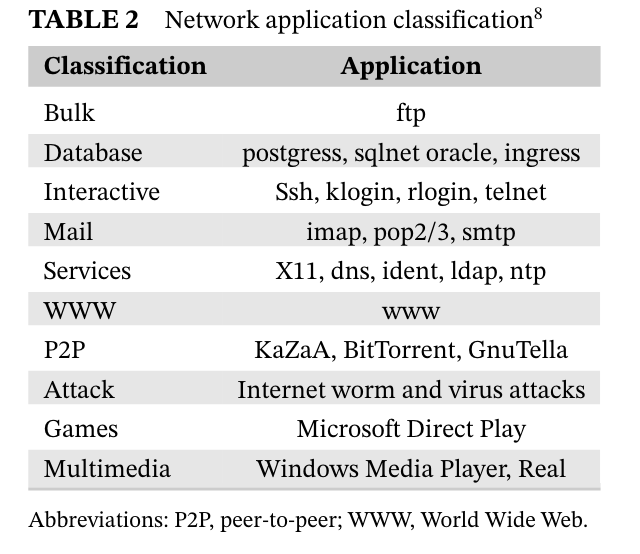
\includegraphics[width=2.5in]{dataset_distribution}
% where an .eps filename suffix will be assumed under latex,
% and a .pdf suffix will be assumed for pdflatex; or what has been declared
% via \DeclareGraphicsExtensions.
\caption{Simulation results for the network.}
\label{fig_sim}
\end{figure}


\cite{}
We evaluate the proposed deep learning–based application classification method on the real-world traffic data set. We
select the Moore data set for testing the application classification method, which is obtained from the computer laboratory
in the University of Cambridge and has been widely used in many traffic classification research works.
2,6,8,23,34
The data
set is composed of 10 separate data sets collected in the different period of a day, and each data set is only composed
of TCP traffic flows. In each data set, for any TCP traffic flow, its 248 flow features such as the size of flow and the
duration time of flow and the corresponding application class label are recorded. All network flows are categorized into
10 classes (ie, World Wide Web (WWW), Mail, Bulk, Services, peer-to-peer (P2P), Database, Attack, Interactive, Games,
and Multimedia). The traffic classification and the corresponding network applications are summarized in Table 2.
Furthermore, to keep the balance of the sample data set, we delete the corresponding 2 types of application samples
from the 10 data sets because the sample numbers of Games and Interactive are relatively small. Moreover, to make the
data set more uniform and to get more accurate simulation results, we randomly select sample data from the 10 data sets
and classify all the network applications into 10 classes (ie, WWW, Mail, File Transfer Protocol (FTP)–control, FTP-pasv,
Attack, P2P, Database, FTP-data, Multimedia, and Services).

% An example of a floating figure using the graphicx package.
% Note that \label must occur AFTER (or within) \caption.
% For figures, \caption should occur after the \includegraphics.
% Note that IEEEtran v1.7 and later has special internal code that
% is designed to preserve the operation of \label within \caption
% even when the captionsoff option is in effect. However, because
% of issues like this, it may be the safest practice to put all your
% \label just after \caption rather than within \caption{}.
%
% Reminder: the "draftcls" or "draftclsnofoot", not "draft", class
% option should be used if it is desired that the figures are to be
% displayed while in draft mode.
%
%\begin{figure}[!t]
%\centering
%\includegraphics[width=2.5in]{myfigure}
% where an .eps filename suffix will be assumed under latex, 
% and a .pdf suffix will be assumed for pdflatex; or what has been declared
% via \DeclareGraphicsExtensions.
%\caption{Simulation results for the network.}
%\label{fig_sim}
%\end{figure}

% Note that the IEEE typically puts floats only at the top, even when this
% results in a large percentage of a column being occupied by floats.
% However, the Computer Society has been known to put floats at the bottom.


% An example of a double column floating figure using two subfigures.
% (The subfig.sty package must be loaded for this to work.)
% The subfigure \label commands are set within each subfloat command,
% and the \label for the overall figure must come after \caption.
% \hfil is used as a separator to get equal spacing.
% Watch out that the combined width of all the subfigures on a 
% line do not exceed the text width or a line break will occur.
%
%\begin{figure*}[!t]
%\centering
%\subfloat[Case I]{\includegraphics[width=2.5in]{box}%
%\label{fig_first_case}}
%\hfil
%\subfloat[Case II]{\includegraphics[width=2.5in]{box}%
%\label{fig_second_case}}
%\caption{Simulation results for the network.}
%\label{fig_sim}
%\end{figure*}
%
% Note that often IEEE papers with subfigures do not employ subfigure
% captions (using the optional argument to \subfloat[]), but instead will
% reference/describe all of them (a), (b), etc., within the main caption.
% Be aware that for subfig.sty to generate the (a), (b), etc., subfigure
% labels, the optional argument to \subfloat must be present. If a
% subcaption is not desired, just leave its contents blank,
% e.g., \subfloat[].


% An example of a floating table. Note that, for IEEE style tables, the
% \caption command should come BEFORE the table and, given that table
% captions serve much like titles, are usually capitalized except for words
% such as a, an, and, as, at, but, by, for, in, nor, of, on, or, the, to
% and up, which are usually not capitalized unless they are the first or
% last word of the caption. Table text will default to \footnotesize as
% the IEEE normally uses this smaller font for tables.
% The \label must come after \caption as always.
%
%\begin{table}[!t]
%% increase table row spacing, adjust to taste
%\renewcommand{\arraystretch}{1.3}
% if using array.sty, it might be a good idea to tweak the value of
% \extrarowheight as needed to properly center the text within the cells
%\caption{An Example of a Table}
%\label{table_example}
%\centering
%% Some packages, such as MDW tools, offer better commands for making tables
%% than the plain LaTeX2e tabular which is used here.
%\begin{tabular}{|c||c|}
%\hline
%One & Two\\
%\hline
%Three & Four\\
%\hline
%\end{tabular}
%\end{table}


% Note that the IEEE does not put floats in the very first column
% - or typically anywhere on the first page for that matter. Also,
% in-text middle ("here") positioning is typically not used, but it
% is allowed and encouraged for Computer Society conferences (but
% not Computer Society journals). Most IEEE journals/conferences use
% top floats exclusively. 
% Note that, LaTeX2e, unlike IEEE journals/conferences, places
% footnotes above bottom floats. This can be corrected via the
% \fnbelowfloat command of the stfloats package.


\section{Discussions}
\subsection{Compare with related work}

\subsection{Limitations}

\section{Conclusion}\label{ch:first}
The conclusion goes here \ref{ch:first}.

\cite{Wang2017}
\cite{Taylor2018}
\cite{Shen2017}

% if have a single appendix:
%\appendix[Proof of the Zonklar Equations]
% or
%\appendix  % for no appendix heading
% do not use \section anymore after \appendix, only \section*
% is possibly needed

% use appendices with more than one appendix
% then use \section to start each appendix
% you must declare a \section before using any
% \subsection or using \label (\appendices by itself
% starts a section numbered zero.)
%


\appendices
\section{Proof of the First Zonklar Equation}
Appendix one text goes here.

%% you can choose not to have a title for an appendix
%% if you want by leaving the argument blank
%\section{}
%Appendix two text goes here.


% use section* for acknowledgment
\ifCLASSOPTIONcompsoc
  % The Computer Society usually uses the plural form
  \section*{Acknowledgments}
\else
  % regular IEEE prefers the singular form
  \section*{Acknowledgment}
\fi


The authors would like to thank...


% Can use something like this to put references on a page
% by themselves when using endfloat and the captionsoff option.
\ifCLASSOPTIONcaptionsoff
  \newpage
\fi



% trigger a \newpage just before the given reference
% number - used to balance the columns on the last page
% adjust value as needed - may need to be readjusted if
% the document is modified later
%\IEEEtriggeratref{8}
% The "triggered" command can be changed if desired:
%\IEEEtriggercmd{\enlargethispage{-5in}}

% references section

% can use a bibliography generated by BibTeX as a .bbl file
% BibTeX documentation can be easily obtained at:
% http://mirror.ctan.org/biblio/bibtex/contrib/doc/
% The IEEEtran BibTeX style support page is at:
% http://www.michaelshell.org/tex/ieeetran/bibtex/
\bibliographystyle{bibtex/IEEEtran}
% argument is your BibTeX string definitions and bibliography database(s)
%\bibliography{../bibtex/IEEEabrv,../bibtex/IEEEbib-July15}
\bibliography{bibtex/IEEEbib-July15}
%
%% <OR> manually copy in the resultant .bbl file
%% set second argument of \begin to the number of references
%% (used to reserve space for the reference number labels box)
%\begin{thebibliography}{1}
%
%\bibitem{IEEEhowto:kopka}
%H.~Kopka and P.~W. Daly, \emph{A Guide to \LaTeX}, 3rd~ed.\hskip 1em plus
%  0.5em minus 0.4em\relax Harlow, England: Addison-Wesley, 1999.
%  
%\end{thebibliography}

% biography section
% 
% If you have an EPS/PDF photo (graphicx package needed) extra braces are
% needed around the contents of the optional argument to biography to prevent
% the LaTeX parser from getting confused when it sees the complicated
% \includegraphics command within an optional argument. (You could create
% your own custom macro containing the \includegraphics command to make things
% simpler here.)
%\begin{IEEEbiography}[{\includegraphics[width=1in,height=1.25in,clip,keepaspectratio]{mshell}}]{Michael Shell}
% or if you just want to reserve a space for a photo:
%
%\begin{IEEEbiography}{Michael Shell}
%Biography text here.
%\end{IEEEbiography}
%
%% if you will not have a photo at all:
%\begin{IEEEbiographynophoto}{John Doe}
%Biography text here.
%\end{IEEEbiographynophoto}
%
%% insert where needed to balance the two columns on the last page with
%% biographies
%%\newpage
%
%\begin{IEEEbiographynophoto}{Jane Doe}
%Biography text here.
%\end{IEEEbiographynophoto}
%
%% You can push biographies down or up by placing
%% a \vfill before or after them. The appropriate
%% use of \vfill depends on what kind of text is
%% on the last page and whether or not the columns
%% are being equalized.

%\vfill

% Can be used to pull up biographies so that the bottom of the last one
% is flush with the other column.
%\enlargethispage{-5in}



% that's all folks
\end{document}


